\documentclass{article}
\usepackage{graphicx} % Required for inserting images
\usepackage[T2A]{fontenc}
\usepackage[english, russian]{babel}
\usepackage{amsfonts}
\usepackage{amsmath}
\usepackage[left=2cm,right=2cm,
    top=2cm,bottom=2cm,bindingoffset=0cm]{geometry}

\setlength\parindent{1.5em}


\title{Домашнее задание 1 (линал)}
\author{Андрей Зотов}
\date{Июнь 2023}
\begin{document}

\maketitle

\section*{Задача 1}
{\bf Ответ:} $y,\ t \in \mathbb{R}$ (свободные переменные);   $x=-2y-t-1,\ z=t$ (главные переменные).
\\
\\
{\bf Решение.} Составим расширенную матрицу СЛУ и решим систему методом Гаусса.
\\
$\left(
    \begin{array}{rrrr|r}
    6 & 12 &  5 &  1 & -6\\
    9 & 18 & 17 & -8 & -9\\ 
    5 & 10 &  4 &  1 & -5
    \end{array}
\right) \Leftrightarrow 
\left(
    \begin{array}{rrrr|r}
    6 & 12 &  5 &  1 & -5\\
    3 &  6 & 12 & -9 & -3\\
    5 & 10 &  4 &  1 & -5
    \end{array}
\right) \Leftrightarrow
\left(
    \begin{array}{rrrr|r}
    1 &  2 &  1 &  0 & -1\\
    3 &  6 & 12 & -9 & -3\\
    5 & 10 &  4 &  1 & -5
    \end{array}
\right) \Leftrightarrow
\left(
    \begin{array}{rrrr|r}
    1 & 2 &  1 &  0 & -1\\
    3 & 6 & 12 & -9 & -3\\
    2 & 4 & -8 & 10 & -2
    \end{array}
\right) \Leftrightarrow
\left(
    \begin{array}{rrrr|r}
    1 & 2 &   1 &  0 & -1\\
    0 & 0 &   9 & -9 &  0\\
    0 & 0 & -10 & 10 &  0
    \end{array}
\right) \Leftrightarrow
\left(
    \begin{array}{rrrr|r}
    1 & 2 &   1 &  0 & -1\\
    0 & 0 &  -1 &  1 &  0\\
    0 & 0 & -10 & 10 &  0
    \end{array}
\right) \Leftrightarrow
\left(
    \begin{array}{rrrr|r}
    1 & 2 &   1 &   0 & -1\\
    0 & 0 &  -1 &   1 &  0\\
    0 & 0 &  10 & -10 &  0
    \end{array}
\right) \Leftrightarrow
\left(
    \begin{array}{rrrr|r}
     1 & 2 &   1 &   0 & -1\\
     0 & 0 &  -1 &   1 &  0\\
     0 & 0 &   0 &   0 &  0
    \end{array}
\right) \Leftrightarrow
\left(
    \begin{array}{rrrr|r}
     1 & 2 &  1 & 0 & -1\\
     0 & 0 & -1 & 1 &  0
    \end{array}
\right) \Leftrightarrow
\left(
    \begin{array}{rrrr|r}
     1 & 2 & 0 &  1 & -1\\
     0 & 0 & 1 & -1 &  0
    \end{array}
\right)$
\\
\par
Получили матрицу канонического ступенчатого вида, из которого следует, что решение СЛУ будет $y,t \in \mathbb{R}$ (свободные переменные) и $x=-2y-t-1,\ z=t$ (главные переменные).
\section*{Задача 2}
{\bf Ответ:} искомый многочлен: $f(x)=x^3+2x^2-7x+5$.
\\
\\
{\bf Решение.} Пусть $f(x)=ax^3+bx^2+cx+d$, тогда $a,b,c,d$ будут корнями СЛУ:
$$
\left\{
   \begin{array}{ccccccccccc}
           a & + &  b & + &  c & + & d & = &  f(1) & = & 1\\
          -a & + &  b & - &  c & + & d & = & f(-1) & = & 13\\
          8a & + & 4b & + & 2c & + & d & = &  f(2) & = & 7\\
        -27a & + & 9b & - & 3c & + & d & = & f(-3) & = & 17       
   \end{array}
\right.
$$
\par
Решим эту систему с помощью метода Гаусса.
\\
\\
$\left(
    \begin{array}{rrrr|r}
      1 & 1 &  1 & 1 & 1\\
     -1 & 1 & -1 & 1 & 13\\
      8 & 4 &  2 & 1 & 7\\
    -27 & 9 & -3 & 1 & 17
    \end{array}
\right) \Leftrightarrow
\left(
    \begin{array}{rrrr|r}
      1 & 1 & 1 & 1 & 1\\
      0 & 1 & 0 & 1 & 7\\
      8 & 4 & 2 & 1 & 7\\
    -27 & 9 & -3 & 1 & 17 
    \end{array} 
\right) \Leftrightarrow
\left(
    \begin{array}{rrrr|r}
      1 & 1 & 1 & 1 & 1\\
      0 & 1 & 0 & 1 & 7\\
      0 & 4 & 6 & 7 & 1\\
    -27 & 9 & -3 & 1 & 17  
    \end{array}  
\right) \Leftrightarrow
\left(
    \begin{array}{rrrr|r}
      1 &  1 & 1  &  1 &  1\\
      0 &  1 & 0  &  1 &  7\\
      0 &  4 & 6  &  7 &  1\\
      0 & 36 & 24 & 28 & 44 
    \end{array}
\right) \Leftrightarrow
\left(
    \begin{array}{rrrr|r}
      1 & 1 & 1 & 1 &  1\\
      0 & 1 & 0 & 1 &  7\\
      0 & 0 & 2 & 1 & -9\\
      0 & 9 & 6 & 7 & 11 
    \end{array}    
\right) \Leftrightarrow
\left(
    \begin{array}{rrrr|r}
      1 & 1 &  1 &  1 &  1\\
      0 & 1 &  0 &  1 &  7\\
      0 & 0 &  2 &  1 & -9\\
      0 & 0 &  6 & -2 & -52 
    \end{array}    
\right) \Leftrightarrow
\left(
    \begin{array}{rrrr|r}
      1 & 1 & 1 &  1 &  1\\
      0 & 1 & 0 &  1 &  7\\
      0 & 0 & 2 &  1 & -9\\
      0 & 0 & 3 & -1 & -26 
    \end{array}    
\right) \Leftrightarrow
\left(
    \begin{array}{rrrr|r}
      1 & 1 & 1 &  1 &  1\\
      0 & 1 & 0 &  1 &  7\\
      0 & 0 & 2 &  1 & -9\\
      0 & 0 & 1 & -2 & -17 
    \end{array}    
\right) \Leftrightarrow
\left(
    \begin{array}{rrrr|r}
      1 & 1 & 1 &  1 &   1\\
      0 & 1 & 0 &  1 &   7\\
      0 & 0 & 1 & -2 & -17\\
      0 & 0 & 0 &  1 &  5 
    \end{array}    
\right) \Leftrightarrow
\left(
    \begin{array}{rrrr|r}
      1 & 0 & 1 &  0 &  -6\\
      0 & 1 & 0 &  1 &   7\\
      0 & 0 & 1 & -2 & -17\\
      0 & 0 & 0 &  1 &  5 
    \end{array}    
\right) \Leftrightarrow
\left(
    \begin{array}{rrrr|r}
      1 & 0 & 0 &  2 &  11\\
      0 & 1 & 0 &  1 &   7\\
      0 & 0 & 1 & -2 & -17\\
      0 & 0 & 0 &  1 &  5 
    \end{array}
\right) \Leftrightarrow
\left(
    \begin{array}{rrrr|r}
      1 & 0 & 0 &  0 &  1\\
      0 & 1 & 0 &  0 &  2\\
      0 & 0 & 1 &  0 & -7\\
      0 & 0 & 0 &  1 &  5 
    \end{array}
\right)$
\\
\\
\par
Получили матрицу канонического ступенчатого вида, из которого следует, что СЛУ имеет единственное решение $a=1,\ b=2,\ c=-7,\ d=5$. Т.е. $$f(x)=x^3+2x^2-7x+5.$$
\section*{Задача 3}
{\bf Ответ:} $\left(
    \begin{array}{rr}
      -32 & 23\\
      -12 & -51
    \end{array}
\right)$ 
\\
\\
{\bf Решение.} Вычислим $(2A)^2$: $(2A)^2 = 4A^2=4\left(\begin{array}{rr}1 & 2\\-3 & 0\end{array}\right)^2 = 4\left(\begin{array}{rr}-5 & 2\\-3 & -6\end{array}\right)=\left(\begin{array}{rr}-20 & 8\\-12 & -24\end{array}\right)$
\\
Вычислим $3((BA)^T-E)^2$:
$$BA=\left(\begin{array}{rr}0 & -1\\2 & 1\end{array}\right)\left(\begin{array}{rr}1 & 2\\-3 & 0\end{array}\right)=\left(\begin{array}{rr}3 & 0\\-1 & 4\end{array}\right)$$
$$\Downarrow$$
$$(BA)^T=\left(\begin{array}{rr}3 & -1\\0 & 4\end{array}\right)$$
$$\Downarrow$$
$$(BA)^T-E=\left(\begin{array}{rr}2 & -1\\0 & 3\end{array}\right)$$
$$\Downarrow$$
$$3((BA)^T-E)^2=3\left(\begin{array}{rr}2 & -1\\0 & 3\end{array}\right)^2=3\left(\begin{array}{rr}4 & -5\\0 & 9\end{array}\right)=\left(\begin{array}{rr}12 & -15\\0 & 27\end{array}\right)$$
Таким образом:
$$(2A)^2-3((BA)^T-E)^2=\left(\begin{array}{rr}-20 & 8\\-12 & -24\end{array}\right)-\left(\begin{array}{rr}12 & -15\\0 & 27\end{array}\right)=\left(\begin{array}{rr}-32 & 23\\-12 & -51\end{array}\right)$$
\section*{Задача 4}
{\bf Ответ:} все матрицы вида $\lambda\left(\begin{array}{rr}-6 & 3\\2 & 0\end{array}\right)$, где $\lambda\in\mathbb{R}$
\\
\\
{\bf Решение.} Пусть $X$ искомая матрица, тогда
\begin{equation}
\label{eq1}
    X\left(\begin{array}{rr}-1 & 3\\2 & 5\end{array}\right)=\left(\begin{array}{rr}-1 & 3\\2 & 5\end{array}\right)X
\end{equation}
\\
Отсюда следует, что $X$ имеет размер $2\times 2$. Тогда будем искать $X$ в виде 
$$\left(\begin{array}{rr}x & y\\z & t\end{array}\right).$$
И из выражения~(\ref{eq1}) получаем, что $x,y,z,t$ являются решениями системы:
$$\begin{cases}-x+3z=-x+2y\\2y+5t=3z+5t\\-y+3t=3x+5y\\2x+5z=-z+2t\end{cases}$$
$$\Updownarrow$$
\begin{equation}
\label{eq2}
    \begin{cases}3z=2y\\2y=3z\\6y+3x+3t=0\\6z+2x-2t=0\end{cases}
\end{equation}
Если поделить на 3 третье уравнение и на 2 четвертое, а также исключить второе уравнение т.к. оно эквивалентно первому, то система~(\ref{eq2}) будет равносильна
\begin{equation}
\label{eq3}
    \begin{cases}3z=2y\\2y+x+t=0\\3z+x-t=0\end{cases}
\end{equation}
Если, учитывая, что  $3z=2y$, вычесть из второго уравнения третье, то получим $t=0$. И переписав второе уравнение, с учетом $t=0$, получим, что система~(\ref{eq3}) равносильна
\begin{equation}
\label{eq4}
    \begin{cases}3z=2y\\x=-2y\\t=0\end{cases}
\end{equation}
А система~(\ref{eq4}), очевидно, равносильна
$$\begin{cases}y\in \mathbb{R}\ \textrm{(свободная переменная)}\\z=\frac{2}{3}y\\x=-2y\\t=0\end{cases}$$
Таким образом $X=\left(\begin{array}{rr}-2y & y\\\frac{2}{3}y & 0\end{array}\right)=\frac{y}{3}\left(\begin{array}{rr}-6 & 3\\2 & 0\end{array}\right)$, где $y\in\mathbb{R}$.
\\
Что равносильно
$$X=\lambda\left(\begin{array}{rr}-6 & 3\\2 & 0\end{array}\right),\ \textrm{где }\lambda\in\mathbb{R}$$
\section*{Задача 5}
{\bf Ответ:} два варианта:
$$CBFDA=\left(\begin{array}{ccccc}1 & 4 & -3 & 2 & 2\\137 & 16 & 65 & -34 & -6\end{array}\right);$$
$$DCBFA=\left(\begin{array}{ccccc}-35 & -7 & -14 & 7 & 0\\-1 & 15 & -14 & 9 & 8\end{array}\right).$$
\\
\\
{\bf Решение.} Рассмотрим ориентированный граф $G$, вершины которого будут данные матрицы $A, B, C, D, F$. При этом наличие ориентированного ребра из вершины $X$ в вершину $Y$ будет означать, что имеет смысл произведение матриц $XY$. Учитывая размеры всех матриц, получим ориентированный граф $G$ (см. рисунок).
\\
{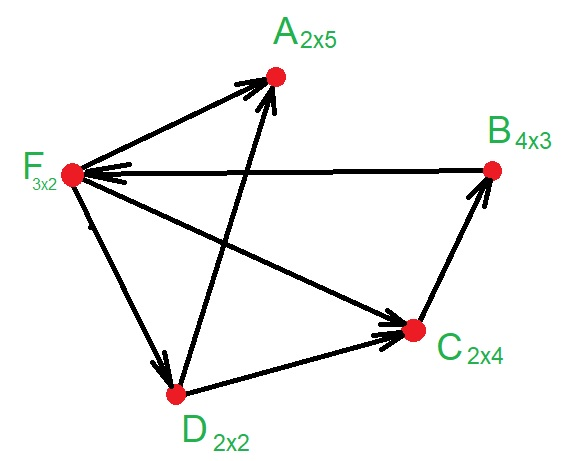
\includegraphics[scale=0.4]{img/img1.jpg}}
\\
\par
Тогда решение задачи будет равносильно нахождению путей в графе $G$, которые содержат каждую вершину ровно один раз. Найдем все такие пути.
\par
Очевидно, если такие пути существуют, то они заканчиваются вершиной $A$, т.к. у вершины $A$ нет исходящих ребер, т.е. такие пути не могут начинаться с вершины $A$. Поэтому возможны 4 случая:
\par
1. Путь начинается с вершины $B$. Далее путь продолжается единственным образом в вершину $F$. Затем путь можно продолжить либо в вершину $A$, либо в вершину $D$, либо в вершину $C$, но $A$ - это тупик, а из вершины $C$ можно попасть только в вершину $B$, из которой мы начали, поэтому путь продолжается единственным образом в вершину $D$. Далее опять возможны два варианта продолжения: либо в $A$, либо в $C$, поэтому единственное продолжение это вершина $C$. Но как уже было замечено из вершины $C$ путь можно продолжить только в вершину $B$, c которой мы начали, при этом вершина $A$ осталась не посещенной. Таким образом путь не может начинаться с вершины~$B$.
\par
2. Путь начинается с вершины $C$. Далее путь продолжается единственны образом в вершину $B$. Затем следует единственное продолжение в вершину $F$. Далее возможны варианты продолжения: $A$ (тупик и вершина $D$ останется не посещенной), $C$ (с этой вершины начали) и $D$, поэтому единственное продолжение это вершина $D$. И завершаем единственным продолжением в вершину $A$. Таким образом возможен путь (или перемножение матриц в этом порядке): $C,B,F,D,A$.
\par
3. Путь начинается с вершины $D$. Далее либо $A$ (тупик), либо $C$, поэтому продолжаем в $C$. Затем единственное продолжение в $B$. Далее единственное продолжение в $F$. И далее завершение пути в $A$. Таким образом возможен путь (или перемножение матриц в этом порядке): $D,C,B,F,A$.
\par
4. Путь начинается с вершины $F$. Далее либо $A$ (тупик), либо $D$, либо $C$, но, как и продолжение в $A$ продолжение в $D$ не образует требуемый путь, т.к. в $A$ можно попасть только из $F$ и $D$ и следовательно попав в $D$ обязательно нужно двигаться в $A$ (в $F$ мы уже побывали), а тогда вершины $B$ и $C$ никогда не будут посещены. Таким образом единственное продолжение из $F$ будет продолжение в $C$. Далее единственное продолжение в $B$. И затем единственное продолжение в вершину $F$, из которой мы стартовали. Таким образом путь не может начинаться с вершины~$F$.
\par
В итоге существует только два возможных порядка перемножения матриц $CBFDA$ и $DCBFA$. Найдем результаты этих перемножений.
\par
Вычислим $CBFDA$:
$$P_1=CB=\left(\begin{array}{ccc}1 & 0 & 3\\-5 & -2 & 7\end{array}\right)$$
$$P_2=P_1F=\left(\begin{array}{cc}-1 & 4\\3 & 16\end{array}\right)$$
$$P_3=P_2D=\left(\begin{array}{cc}0 & 1\\28 & -3\end{array}\right)$$
$$CBFDA=P_3A=\left(\begin{array}{ccccc}1 & 4 & -3 & 2 & 2\\137 & 16 & 65 & -34 & -6\end{array}\right)$$
\par
Вычислим $DCBFA$:
$$Q_1=DC=\left(\begin{array}{cccc}7 & 8 & -5 & -2\\1 & 2 & -1 & 0\end{array}\right)$$
$$Q_2=Q_1B=\left(\begin{array}{ccc}9 & 2 & 5\\1 & 0 & 3\end{array}\right)$$
$$Q_3=Q_2F=\left(\begin{array}{cc}-7 & 0\\-1 & 4\end{array}\right)$$
$$DCBFA=Q_3A=\left(\begin{array}{ccccc}-35 & -7 & -14 & 7 & 0\\-1 & 15 & -14 & 9 & 8\end{array}\right)$$
\end{document}

